%!TEX program = xelatex
\documentclass[master,oldfontcfg,euler,twoside,openany]{cugthesis}
% 默认twoside 双面打印
% 将master修改为bachelor, doctor or master (暂时只支持硕士毕业论文模版)
% 要使用adobe字体,添加adobefonts选项
% 使用euler数学字体,如不愿使用,去掉euler
% 使用外文写作,请添加notchinese
% oldfontcfg,使用老板的字体设置,建议初学者开启

% 设置图形文件的搜索路径
\graphicspath{{figures/}}
\newcommand{\tabincell}[2]{\begin{tabular}{@{}#1@{}}#2\end{tabular}}
%仅用于本示例文档中显示特殊字符串
\usepackage{xltxtra}
%仅用于子图
%\usepackage{graphicx}
%\usepackage{subfigure}

%%%%%%%%%%%%%%%%%%%%%%%%%%%%%%
%% 封面部分
%%%%%%%%%%%%%%%%%%%%%%%%%%%%%%

  % 中文封面内容
  \title{MapReduce中间结果重用优化及分析}%一般情况下扉页和封皮、书脊共用一个标题文本,可以不用定义\spinetitle(仅硕博有用), \covertitle(本硕博均有用)和\encovertitle(仅本科有用)。特殊情况见下。
  \spinetitle{MapReduce中间结果重用优化及分析}
  %特殊情况1:本例中\title命令里含有换行控制字符,这会导致制作书脊的时候出现错误,例如如果你注释掉\spinetitle{...}这一行就会报错。这时需要定义一个不含换行等命令的\spinetitle,这并不表示\spinetitle里不能有任何命令——只能使用有限的命令。
  %特殊情况2:本例中标题过长,所以需要缩小书脊标题的字号。
  %特殊情况3:本例中中英文混排,由于tex竖排的原理限制,中英文基线不重合,所以需要人工调整英文的基线。具体调整量根据不同字体有所不同。
  \covertitle{MapReduce中间结果重用优化及分析}
  %\covertitle{中文题目第一行\\中文题目第二行}
  %不要在此调整封皮字体大小! Do not set Cover Page font size here!
  %特殊情况4:本例中\title中含有多个换行,导致标题超过了两行。根据制本厂规定,封皮标题不能超过两行。因此需要定义封皮使用的标题\covertitle. 如果你注释掉这一行,就会发现封皮不符合规定。
  \encovertitle{MapReduce Performance Acceleration and Analytics with Intermediate Results Reusing}
  %\encovertitle{English Title Line 1\\English Title Line 2\\English Title Line 3}
  %不要在此调整封皮字体大小! Do not set Cover Page font size here!
  %特殊情况5:仅本科生有用。本科封皮中有英文标题,不超过三行。与上类似。

  \author{徐\ 锦\ 来}
  \depart{信息工程学院}%系别,硕博请用系代号,本科请用全称如
  %\depart{数理化和信息工程系}
  \major{软件工程专业}%专业,硕博请用全称,本科不需要
  \advisor{罗忠文\ 教授}
  %\coadvisor{姚宏\ 教授}%第二导师,没有请注释掉
  \studentid{120121352}%
  \submitdate{二〇一五年五月}
  %\numsubmitdate{2015.04}
  % 英文封面内容
  \entitle{MapReduce Performance Acceleration and Analytics \\with Intermediate Results Reusing}
  \enauthor{Jinlai Xu}
  \enmajor{Software Engineering}
  \enadvisor{Prof. Zhongwen Luo}
  %\encoadvisor{Prof. Hong Yao}%另外一个导师
  \ensubmitdate{2015.05}
  
%%%%%%%%%%%%%%%%%%%%%%%%%%%%%%%%%%%%%%%%%%%%%%%%%%%%%%%%%%%%%%%%%%%%%
% If you use another language instead of chinese and english, then you
% should define some strings and provide information in your language.
%%%%%%%%%%%%%%%%%%%%%%%%%%%%%%%%%%%%%%%%%%%%%%%%%%%%%%%%%%%%%%%%%%%%%
%  \otherustcstr{zhong guo ke xue ji shu da xue}%A translation of `University of Science and Technology of China' in your language
%  \otherthesisstr{shuo shi xue wei lun wen}%A translation of `A dissertation for doctor(master/bachelor)'s degree' in your language
%  \otherauthorstr{xing ming}%A translation of `Author' in your language
%  \otherdepartmentstr{yuan xi}%A translation of `Department' in your language
%  \otherstudentidstr{xue hao}%A translation of `Student ID' in your language
%  \othersupervisorstr{dao shi}%A translation of `Supervisor' in your language
%  \otherfinishedtimestr{ri qi}%A translation of `Finished Time' in your language
%  \otherspecialitystr{zhuan ye}%A translation of `Speciality' in your language
%  \othertitle{zhong guo ke xue ji shu da xue tong yong xue wen lun wen shi li wen dang}
%  \otherauthor{zhao qian sun}
%  \otheradvisor{zhou wu zheng}
%  \othercoadvisor{feng chen zhu}
%  \othersubmitdate{hou nian ma yue}
%  \othermajor{mou zhuan ye}
%  \otherdepart{mou xi}

\begin{document}

  % 封面
  \maketitle

%特别注意,以下述顺序为准,在对应部分添加文档部件,切勿颠倒顺序:
%本科论文的文档部件顺序是:
%    frontmatter:致谢、目录、中文摘要、英文摘要、
%    mainmatter: 正文章节
%    backmatter: 参考文献或资料注释、附录
%硕博论文的文档部件顺序是:
%    frontmatter:中文摘要、英文摘要、目录、符号说明
%    mainmatter: 正文章节
%    backmatter: 参考文献、附录、致谢、发表论文
%%%%%%%%%%%%%%%%%%%%%%%%%%%%%%
%% 前言部分
%%%%%%%%%%%%%%%%%%%%%%%%%%%%%%
\frontmatter
%\pagenumbering{}
\makeatletter
\ifustc@bachelor
	%%%%%%%%%%%%%%%%%
	%本科论文修改这里
	%%%%%%%%%%%%%%%%%
	% 致谢
	% !TEX root = ../main.tex
\begin{thanks}

感谢原中科大本硕博论文模版的制作人员

包括但不限于ywg,XPS,Liuqs,Guolicai,刘青松等原模版的制作者和维护者

我在这里只是按照中国地质大学的work版本的硕士论文模版进行了一定的修改

以满足使用\LaTeX 撰写中国地质大学硕士论文的目的

感谢大家对本模板更新工作的支持!

本模板以及本示例文档还存在许多不足之处,欢迎大家测试并及时提供反馈。

\begin{flushright}
seeksky@CUG

欢迎访问我的博客 http://jinlaixu.net
\end{flushright}


在中国地质大学完成本科和硕士连读学业的七年里,我所从事的学习和研究工作,都是在导师以及系里其他老师和同学的指导和帮助下进行的。在完成论文之际,请容许我对他们表达诚挚的谢意。

首先感谢导师XXX教授和XXX副教授多年的指导和教诲,是他们把我带到了计算机视觉的研究领域。X老师严谨的研究态度及忘我的工作精神,X老师认真细致的治学态度及宽广的胸怀,都将使我受益终身。

感谢班主任XXX老师和XX老师多年的关怀。感谢XXX、XX、XX等老师,他们本科及研究生阶段的指导给我研究生阶段的研究工作打下了基础。

感谢XX、XXX、XXX、XX、XXX、XXX、XXX、XX等师兄师姐们的指点和照顾;感谢XXX、XX、XXX等几位同班同学,与你们的讨论使我受益良多;感谢XXX、XX、XXX、XX、XXX等师弟师妹,我们在XXX实验室共同学习共同生活,一起走过了这段愉快而难忘的岁月。

感谢科大,感谢一路走过来的兄弟姐妹们,在最宝贵年华里,是你们伴随着我的成长。

最后,感谢我家人一贯的鼓励和支持,你们是我追求学业的坚强后盾。

\vskip 18pt

\begin{flushright}

~~~~赵钱孙~~~~

\today

\end{flushright}

\end{thanks}

	
	%目录部分
	%目录
	\tableofcontents
	%默认表格、插图、算法索引名称分别为“表格索引”、“插图索引”和“算法索引”
	%如果需要自行修改lot,lof,loa的名称,请定义
	%\ustclotname{...}
	%\ustclofname{...}
	%\ustcloaname{...}

	% 表格索引
	\ustclot
	% 插图索引
	\ustclof
	%算法索引 
	%如果需要使用算法环境并列出算法索引,请加入补充宏包。
	\ustcloa
	
	% 摘要
	% Abstract
\clearpage
\thispagestyle{plain}
\phantomsection
\addcontentsline{toc}{chapter}{Abstract}

\centerline{\zihao{3}\bfseries Abstract}

\linespread{1.4}\zihao{-4}
\bigskip

This thesis explores the relationship between focus structure and pronoun resolution among non-native speakers of English and French. Firstly we reviewed the existing literature on the mechanism of focus effect and pronoun resolution. Then through a self-paced reading test, we find that focus, in the form of cleft structure does not necessarily increase the salience of a informational unit, thus may not in some cases make it a preferred antecedent for pronoun resolution. This result is line with previous researches on this topic. In our experiment, We also find that focused subject in French and focused object in English are processed faster, but focused subjects in both languages leads to longer response time of anaphora. Furthermore, our research also shows that the congruence between anaphora and focus does not make the latter more accessible. In this regard, we argue that the problem of whether there is subject or object preference in English and French is more complicated than the results of current studies.

\bigskip
\noindent\textbf{\zihao{4} Keywords:} 
focus effect, pronoun resolution, self-paced reading, English, French

%此文件中含有中英文摘要
\else
	%%%%%%%%%%%%%%%%%
	%硕博论文修改这里
	%%%%%%%%%%%%%%%%%
  % 个人简介
  \resumeitem{个人简历:}
\noindent xxxx 年 xx 月 xx 日出生于 xx 省 xx 县。\\
\noindent xxxx 年 9 月考入 xx 大学 xx 系 xx 专业,xxxx 年 7 月本科毕业并获得 xx 学士学位。\\
\noindent xxxx 年 9 月免试进入 xx 大学 xx 系攻读 xx 学位至今。

\resumeitem{发表论文:} % 发表的和录用的合在一起
\begin{enumerate}[{[}1{]}]
\item Yang Y, Ren T L, Zhang L T, et al. Miniature microphone with silicon-
  based ferroelectric thin films. Integrated Ferroelectrics, 2003,
  52:229-235. (SCI 收录, 检索号:758FZ.)
\item 杨轶, 张宁欣, 任天令, 等. 硅基铁电微声学器件中薄膜残余应力的研究. 中国机
  械工程, 2005, 16(14):1289-1291. (EI 收录, 检索号:0534931 2907.)
\item 杨轶, 张宁欣, 任天令, 等. 集成铁电器件中的关键工艺研究. 仪器仪表学报,
  2003, 24(S4):192-193. (EI 源刊.)
\item Yang Y, Ren T L, Zhu Y P, et al. PMUTs for handwriting recognition. In
  press. (已被 Integrated Ferroelectrics 录用. SCI 源刊.)
\item Wu X M, Yang Y, Cai J, et al. Measurements of ferroelectric MEMS
  microphones. Integrated Ferroelectrics, 2005, 69:417-429. (SCI 收录, 检索号
  :896KM.)
\item 贾泽, 杨轶, 陈兢, 等. 用于压电和电容微麦克风的体硅腐蚀相关研究. 压电与声
  光, 2006, 28(1):117-119. (EI 收录, 检索号:06129773469.)
\item 伍晓明, 杨轶, 张宁欣, 等. 基于MEMS技术的集成铁电硅微麦克风. 中国集成电路, 
  2003, 53:59-61.
\end{enumerate}

\resumeitem{研究成果:} % 有就写,没有就删除
\begin{enumerate}[{[}1{]}]
\item 任天令, 杨轶, 朱一平, 等. 硅基铁电微声学传感器畴极化区域控制和电极连接的
  方法: 中国, CN1602118A. (中国专利公开号.)
\item Ren T L, Yang Y, Zhu Y P, et al. Piezoelectric micro acoustic sensor
  based on ferroelectric materials: USA, No.11/215, 102. (美国发明专利申请号.)
\end{enumerate}

  % 摘要
  % Abstract
\clearpage
\thispagestyle{plain}
\phantomsection
\addcontentsline{toc}{chapter}{Abstract}

\centerline{\zihao{3}\bfseries Abstract}

\linespread{1.4}\zihao{-4}
\bigskip

This thesis explores the relationship between focus structure and pronoun resolution among non-native speakers of English and French. Firstly we reviewed the existing literature on the mechanism of focus effect and pronoun resolution. Then through a self-paced reading test, we find that focus, in the form of cleft structure does not necessarily increase the salience of a informational unit, thus may not in some cases make it a preferred antecedent for pronoun resolution. This result is line with previous researches on this topic. In our experiment, We also find that focused subject in French and focused object in English are processed faster, but focused subjects in both languages leads to longer response time of anaphora. Furthermore, our research also shows that the congruence between anaphora and focus does not make the latter more accessible. In this regard, we argue that the problem of whether there is subject or object preference in English and French is more complicated than the results of current studies.

\bigskip
\noindent\textbf{\zihao{4} Keywords:} 
focus effect, pronoun resolution, self-paced reading, English, French

%此文件中含有中英文摘要
	% 目录
	\tableofcontents
	%默认表格、插图、算法索引名称分别为“表格索引”、“插图索引”和“算法索引”
	%如果需要自行修改lot,lof,loa的名称,请定义
	%\ustclotname{...}
	%\ustclofname{...}
	%\ustcloaname{...}

	% 表格索引
	\ustclot
	% 插图索引
	\ustclof
	%算法索引 
	%如果需要使用算法环境并列出算法索引,请加入补充宏包。
	%\ustcloa
	
	%符号说明,需要加入补充包
	\begin{denotation}
\begin{table}[h]%此处最好是h
\caption{国际单位制中具有专门名称的导出单位}
\vspace{0.5em}\centering\wuhao
\begin{tabular}{ccccc}
\toprule[1.5pt]
量的名称&单位名称&单位符号&其它表示实例\\
\midrule[1pt]
频率&赫[兹]&Hz&s-1\\
\bottomrule[1.5pt]
\end{tabular}
\end{table}
\end{denotation}
%不是必需的,如果不想列出请注释掉
\fi
\makeatother

%%%%%%%%%%%%%%%%%%%%%%%%%%%%%%
%% 正文部分
%%%%%%%%%%%%%%%%%%%%%%%%%%%%%%
\mainmatter

  \chapter{Introduction}
\label{chap:intro}

\section{What is Lorem Ipsum?}
\label{sec:apadia}

Lorem Ipsum is simply dummy text of the printing and typesetting industry. Lorem Ipsum has been the industry's standard dummy text ever since the 1500s, when an unknown printer took a galley of type and scrambled it to make a type specimen book \cite{banerjee:pedersen:2003}. It has survived not only five centuries, but also the leap into electronic typesetting, remaining essentially unchanged. It was popularised in the 1960s with the release of Letraset sheets containing Lorem Ipsum passages, and more recently with desktop publishing software like Aldus PageMaker including versions of Lorem Ipsum \cite{berment:phd:2004}.



\section{Where Does It Come From?}
\label{sec:where}

Contrary to popular belief, Lorem Ipsum is not simply random text. It has roots in a piece of classical Latin literature from 45 BC, making it over 2000 years old. Richard McClintock, a Latin professor at Hampden-Sydney College in Virginia, looked up one of the more obscure Latin words, consectetur, from a Lorem Ipsum passage, and going through the cites of the word in classical literature, discovered the undoubtable source \cite{azarova:etal:2002,budanitsky:hirst:2006}. Lorem Ipsum comes from sections 1.10.32 and 1.10.33 of ``de Finibus Bonorum et Malorum'' (The Extremes of Good and Evil) by Cicero, written in 45 BC. This book is a treatise on the theory of ethics, very popular during the Renaissance. The first line of Lorem Ipsum, ``''Lorem ipsum dolor sit amet\ldots'', comes from a line in section 1.10.32.

The standard chunk of Lorem Ipsum used since the 1500s is reproduced below for those interested. Sections 1.10.32 and 1.10.33 from ``de Finibus Bonorum et Malorum'' by Cicero are also reproduced in their exact original form, accompanied by English versions from the 1914 translation by H. Rackham. 

\begin{equation}
-\frac{(x_0 - \mu)^2}{2 \sigma^2} = -\ln 2
\end{equation}


\section{Examples}
\label{sec:examples}

The first few paragraphs of Lorem Ipsum are given below.

\subsection{First Paragraph}

Lorem ipsum dolor sit amet, consectetur adipiscing elit. Donec posuere, neque quis feugiat egestas, quam sapien dictum justo, eu vulputate nunc metus sed dui. Integer molestie leo quis libero facilisis, dictum pretium quam ornare. Vestibulum ante ipsum primis in faucibus orci luctus et ultrices posuere cubilia Curae; Vivamus luctus rutrum magna non convallis. Praesent vestibulum consequat eros, et fringilla nisi suscipit id. Nam vulputate justo dui, eu rutrum est accumsan ut. Sed molestie erat vitae mi blandit, in volutpat urna lobortis. Vestibulum mollis rutrum gravida. Fusce dolor nulla, condimentum vel pretium ut, venenatis eget leo. Ut semper placerat mauris, ut tempus est tempor vel. Interdum et malesuada fames ac ante ipsum primis in faucibus. In vitae feugiat diam. Pellentesque accumsan consequat turpis aliquam elementum.


\subsection{Next Two Paragraphs}

Vivamus dignissim arcu nunc, non aliquam sem porta vitae. Sed sodales accumsan dui sit amet egestas. Maecenas rhoncus a erat eget accumsan. 

\begin{table}[hbt!]\centering
\caption{Number of Jewels}

\begin{tabular}{l c}
\hline
Type & Quantity \\\hline
Sapphire & 6\\
Diamond & 23\\
Gold & 56\\
Silver & 235\\
Bronze & 324\\\hline
\end{tabular}
\end{table}

\begin{itemize}
\item Etiam vitae pulvinar metus, sed fringilla orci. 
\item Duis dapibus dolor risus, non ultrices enim porta sit amet. 
\item Ut eu libero augue. 
\end{itemize}

Nulla ipsum augue, feugiat ac laoreet quis, pretium ut magna. Class aptent taciti sociosqu ad litora torquent per conubia nostra, per inceptos himenaeos. Integer blandit placerat dictum.

\begin{figure}[hbt!]\centering
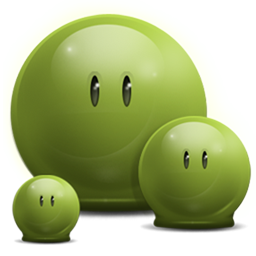
\includegraphics[width=.5\textwidth]{green}
\caption{Example figure}
\end{figure}

Sed dolor justo, scelerisque sed rutrum quis, porttitor a mauris. Cras non auctor felis, rutrum fringilla risus. Integer at convallis erat, sit amet luctus turpis. Duis sed rutrum eros, quis tempus risus. Etiam pellentesque nisi odio, eget dignissim eros ultrices et. Aliquam leo massa, fermentum vel odio sed, ullamcorper molestie lorem. Integer lorem felis, adipiscing sit amet interdum eget, auctor at lorem. Aliquam ultricies tortor eu nibh facilisis tincidunt.


\subsubsection{Some Notes}

Duis sed rutrum eros, quis tempus risus. Etiam pellentesque nisi odio, eget dignissim eros ultrices et. Aliquam leo massa, fermentum vel odio sed, ullamcorper molestie lorem.

\subsubsection{And Further}
Duis sed rutrum eros, quis tempus risus. Etiam pellentesque nisi odio, eget dignissim eros ultrices et. Aliquam leo massa, fermentum vel odio sed, ullamcorper molestie lorem.


\subsection{Least-Squares with Forgetting Factor AdaptiveLaw}

\section{Mechatronic Suspension System; History and a Brief Background}
Nulla ipsum augue, feugiat ac laoreet quis, pretium ut magna. Class aptent taciti sociosqu ad litora torquent per conubia nostra, per inceptos himenaeos. Integer blandit placerat dictum.



\section{Summary}
Nulla ipsum augue, feugiat ac laoreet quis, pretium ut magna. Class aptent taciti sociosqu ad litora torquent per conubia nostra, per inceptos himenaeos. Integer blandit placerat dictum.

Sed dolor justo, scelerisque sed rutrum quis, porttitor a mauris. Cras non auctor felis, rutrum fringilla risus. Integer at convallis erat, sit amet luctus turpis. Duis sed rutrum eros, quis tempus risus. Etiam pellentesque nisi odio, eget dignissim eros ultrices et. Aliquam leo massa, fermentum vel odio sed, ullamcorper molestie lorem. Integer lorem felis, adipiscing sit amet interdum eget, auctor at lorem. Aliquam ultricies tortor eu nibh facilisis tincidunt.
  \include{chapter/chap-analytics}
  \include{chapter/chap-IntermediateAnalysis}
  \include{chapter/chap-memomr}
  \include{chapter/chap-experiment}
  %\include{chapter/chap-application}
  \include{chapter/chap-summary}
  %自行添加
  %\include{chapter/...}

%%%%%%%%%%%%%%%%%%%%%%%%%%%%%%
%% 附件部分
%%%%%%%%%%%%%%%%%%%%%%%%%%%%%%
\backmatter
  \makeatletter
  \ifustc@bachelor\relax\else
    % 致谢
    % !TEX root = ../main.tex
\begin{thanks}

感谢原中科大本硕博论文模版的制作人员

包括但不限于ywg,XPS,Liuqs,Guolicai,刘青松等原模版的制作者和维护者

我在这里只是按照中国地质大学的work版本的硕士论文模版进行了一定的修改

以满足使用\LaTeX 撰写中国地质大学硕士论文的目的

感谢大家对本模板更新工作的支持!

本模板以及本示例文档还存在许多不足之处,欢迎大家测试并及时提供反馈。

\begin{flushright}
seeksky@CUG

欢迎访问我的博客 http://jinlaixu.net
\end{flushright}


在中国地质大学完成本科和硕士连读学业的七年里,我所从事的学习和研究工作,都是在导师以及系里其他老师和同学的指导和帮助下进行的。在完成论文之际,请容许我对他们表达诚挚的谢意。

首先感谢导师XXX教授和XXX副教授多年的指导和教诲,是他们把我带到了计算机视觉的研究领域。X老师严谨的研究态度及忘我的工作精神,X老师认真细致的治学态度及宽广的胸怀,都将使我受益终身。

感谢班主任XXX老师和XX老师多年的关怀。感谢XXX、XX、XX等老师,他们本科及研究生阶段的指导给我研究生阶段的研究工作打下了基础。

感谢XX、XXX、XXX、XX、XXX、XXX、XXX、XX等师兄师姐们的指点和照顾;感谢XXX、XX、XXX等几位同班同学,与你们的讨论使我受益良多;感谢XXX、XX、XXX、XX、XXX等师弟师妹,我们在XXX实验室共同学习共同生活,一起走过了这段愉快而难忘的岁月。

感谢科大,感谢一路走过来的兄弟姐妹们,在最宝贵年华里,是你们伴随着我的成长。

最后,感谢我家人一贯的鼓励和支持,你们是我追求学业的坚强后盾。

\vskip 18pt

\begin{flushright}

~~~~赵钱孙~~~~

\today

\end{flushright}

\end{thanks}
%硕博致谢部分
    % 发表文章目录
    %% !TEX root = ../main.tex
\chapter{在读期间发表的学术论文与取得的研究成果}

\noindent\textbf{研究工作:}

\begin{enumerate}

\item A A A A A A A A A
\item A A A A A A A A A
\item A A A A A A A A A
\item A A A A A A A A A

\end{enumerate}


\noindent\textbf{已发表论文:}

\begin{enumerate}

\item A A A A A A A A A 
\item A A A A A A A A A
\item A A A A A A A A A
\item A A A A A A A A A
\item A A A A A A A A A
\item A A A A A A A A A
\item A A A A A A A A A
\item A A A A A A A A A

\end{enumerate}

\vskip 1cm

\noindent\textbf{待发表论文:}

\begin{enumerate}

\item A A A A A A A A A

\end{enumerate} 
  \fi
  \makeatother
  % 参考文献
  % 使用 BibTeX
  % 选择参考文献的排版格式。注意ustcbib这个格式不保证完全符合要求,请自行决定是否使用
  \bibliographystyle{cugbib}%{GBT7714-2005NLang-UTF8}
  %\bibliographystyle{gbt7714-2005}%{GBT7714-2005NLang-UTF8}
  \bibliography{bib/ref}
  \nocite{*} % for every item
  % 不使用 BibTeX
  % 
\begin{thebibliography}{10}

\bibitem{deng:01a}
{�˽���,~��ȽȽ,~�³���}.
\newblock {\em \LaTeXe{}~�Ƽ��Ű�ָ��}.
\newblock ��ѧ������,~���:~7-03-009239-2/TP.1516, ����, 2001.

\bibitem{wang:00a}
����.
\newblock {\em \LaTeXe{}~��ͼָ��}.
\newblock 2000.

\bibitem{zhang:03a}
���ֲ�.
\newblock {\em �����°�~CCT~��˵��}.
\newblock 2003.

\bibitem{lshort-cn}
C\TeX{} ������.
\newblock {\em lshort~����~3.20}.
\newblock 2003.

\bibitem{knuth86e}
Donald~E. Knuth.
\newblock {\em Computer Modern Typefaces}, volume~E of {\em Computers and
  Typesetting}.
\newblock Addison-Wesley, Reading, Massachusetts, 1986.

\bibitem{knuth86d}
Donald~E. Knuth.
\newblock {\em {METAFONT}: The Program}, volume~D of {\em Computers and
  Typesetting}.
\newblock Addison-Wesley, Reading, Massachusetts, 1986.

\bibitem{knuth86c}
Donald~E. Knuth.
\newblock {\em The {METAFONT}book}, volume~C of {\em Computers and
  Typesetting}.
\newblock Addison-Wesley, Reading, Massachusetts, 1986.

\bibitem{knuth86b}
Donald~E. Knuth.
\newblock {\em {TeX}: The Program}, volume~B of {\em Computers and
  Typesetting}.
\newblock Addison-Wesley, Reading, Massachusetts, 1986.

\bibitem{knuth86a}
Donald~E. Knuth.
\newblock {\em The {TeX}book}, volume~A of {\em Computers and Typesetting}.
\newblock Addison-Wesley, Reading, Massachusetts, 1986.

\bibitem{lamport85a}
Leslie Lamport.
\newblock {\em {LaTeX} --- A Document Preparation System: User's Guide and
  Reference Manual}.
\newblock Addison-Wesley, Reading, Massachusetts, 2nd edition, 1985.

\end{thebibliography}


  % 附录,没有请注释掉
  \begin{appendix}
    % !TEX root = ../main.tex
\chapter{关于硕士、博士学位论文撰写要求}
\label{chap:requires}

学位论文是学位申请者为申请学位而撰写的学术论文,它集中作者在研究工作中获得可行的发明、理论和见解,是评判学位申请人学术水平的重要依据和获得学位的必要条件之一,也是科研领域中的主要文献资料和社会宝贵财富。
为提高研究生学位论文的质量,做到学位论文在内容和格式上规范化与统一化,特作如下规定:

\section{对学位论文的基本要求}

\textbf{一下文字仅作示例,一切以学校规定为准!}

\subsection{硕士学位论文}

根据《中华人民共和国学位条例暂行实施办法》第八条的规定,硕士学位论文应能表明作者确已在本门学科上掌握了坚实的基础理论和系统的专门知识,并对所研究的课题有新的见解,有从事科学研究或独立担负专门技术工作的能力。硕士学位论文工作一般是在硕士生完成培养计划规定的课程学习后开始,其工作内容因学科的性质不同而有所差异,一般包括文献阅读、开题报告、拟定并实施工作计划、科研调查、实验研究、理论分析和文字总结等工作。论文正文一般应不少于3万字。硕士学位论文必须有一定的工作量,在论文题目确定后,用于论文工作的时间一般不应少于1.5年。

\subsection{博士学位论文}

根据《中华人民共和国学位条例暂行实施办法》第十三条的规定,博士学位论文应能表明作者确已在本门学科上掌握了坚实宽广的基础理论和系统深入的专门知识,具有独立从事科学研究工作的能力,并在科学或专门技术工作上做出了创造性的成果。博士学位论文工作是攻读博士学位研究生培养的最重要环节,其工作时间一般应不少于2学年。博士生入学后在导师指导下明确科研方向,收集资料,阅读文献,进行调查研究,确定研究课题。一般在第二至第三学期通过开题报告并制定论文工作计划。博士生应根据论文工作计划分阶段在教研室、学术会议上报告科研和论文工作的进展情况。论文正文一般应不少于5万字。博士生用于论文研究和撰写学位论文的时间一般应不得少于2年。

特别应注意,学位论文应是本人的研究成果,在导师指导下独立完成,不得抄袭或剽窃他人成果。论文应反映作者较好地掌握了本学科、专业的研究方法和技能,学术观点必须言之有理、持之有据,论文内容应层次分明,数据可靠,文字简炼,推理严谨,立论正确。

\section{对学位论文的格式要求}

\subsection{编写要求}

硕士、博士学位论文一般应由以下全部或某几部分组成,依次为:封面、中文摘要、英文摘要 、目录、符号说明、正文、参考文献、附录、附图表、致谢、攻读学位期间发表的学术论文目录。

具体要求如下:

\subsubsection{封面}

采用研究生院规定的统一封面,封面上填写论文题目、作者姓名、导师姓名、学科(专业) 、论文完成时间。上述内容也应在扉页上填写清楚。论文题目采用黑体26磅加粗居中,其他采用宋体16磅居中。书脊用黑体12磅,上方写论文题目,中间写系别,下方写研究生姓名(彩色封面在制信厂或印刷厂装订)。

\subsubsection{论文摘要}

学位论文的中文摘要应以最简洁的语言介绍论文的概要、作者的突出论点、新见解或创造性成果。硕士学位论文中文摘要一般应在500字左右,博士学位论文中文摘要一般在1500字左右。英文摘要(Abstract)内容应与中文摘要基本相对应,要语句通顺,语法正确,能正确概括文章的内容。摘要标题采用黑体16磅居中,正文采用宋体12磅(英文用Times New Roman体12磅),行距20磅。

\subsubsection{正文}

正文是学位论文的主体和核心部分,它是将学习、研究和调查过程中筛选、观察和测试所获得的材料,经过加工整理和分析研究,由材料而形成论点。不同学科、专业有着不同的写作内容,但作为一般要求,论据、论点应力求准确、完备、清晰、通顺,实事求是,客观真切,简短精炼,合乎逻辑。一般标题字体采用黑体14磅,多级标题可采用粗体14磅或粗体12磅。正文字体采用宋体12磅(英文用Times New Roman体12磅),两端对齐书写,行距20磅。


绪论或引言是学位论文主体部分的开端,主要说明研究工作的缘起、沿革、目的、涉及范围 、国内外研究现状、相关领域的前人研究成果和知识空白、理论分析的依据、研究设想、研究方法和实际设计的概述,以及文中拟解决的问题、理论意义和实用价值等,应言简意赅,不要与摘要雷同或成为摘要的解释,也不是提要。

结论是学位论文最终和总体的结论,是整篇论文的归宿,应明确、精炼、完整、准确。要着重阐述作者研究的创造性成果、新见解、新发现和新发展,及其在本研究领域中的地位、作用、价值和意义,还可进一步提出需要讨论的问题和建议。学位论文中的计量单位、制图、制表、公式规范、缩略词和符号必须遵循GB 3100~3102—93(国家技术监督局1993-12-27发布,1994-07-01实施)有关量和单位的规定。如无标准可循,应采用本学科或专业有关权威性机构或学术团体所公布的规定。如不得已必需引用某些未公知公用的、不易为同行读者所理解的或系作者自行拟定的符合、记号、缩略词等,均应一一在第一次出现时加以说明,给以明确的定义。

\subsubsection{参考文献}

参考文献应按文中引用的顺序列出,可以分列在各章末尾,也可以列在正文的末尾。

本着以严谨求实的科学态度撰写论文,凡学位论文中有引用他人成果之处,均应详细列出所引文献的名称、作者、发表刊物、发表时间、卷号、页码等。标题字体采用黑体14磅,正文字体采用宋体10磅(英文用Times New Roman体10磅),行距16磅。

\subsubsection{附录}
主要列入正文内过分冗长的公式推导,供查读方便所需的辅助性数学工具或表格,重复性数据图表,论文使用的缩写,程序全文及说明等。

\subsubsection{致谢}

表达作者对完成论文和学业提供帮助的老师、同学、领导、同事及亲属的感激之情。

\subsubsection{攻读学位期间发表的学术论文目录}

按学术论文发表的时间顺序,列齐本人在攻读学位期间发表或已录用的学术论文清单(发表刊物名称、卷册号、页码、年月及论文署名、作者排序)。

\subsection{打印}

按照有关规定,凡授予中华人民共和国学位者,学位论文必须用中文撰写,同时一律用A4标准纸打印输出,一般应有篇眉。篇眉和页码均采用宋体10磅居中,页面设置上边距3.8cm、下边距为3.0cm,左边距为3.5cm、右边距为3.0cm。

\subsection{装订}

学位论文撰写完成后,用研究生院统一封面线装订成册。所需份数由研究生本人及导师掌握(可参考学位申请上报材料清单的要求)。

  \end{appendix}

  

  

\end{document}
